\documentclass[twocolumn]{article}

\usepackage{lipsum} 
\usepackage{hyperref}
\usepackage{placeins}
%\hypersetup{colorlinks,urlcolor=blue}
\hypersetup{colorlinks,urlcolor=black}

\usepackage{graphicx}

\title{Habitat Connectivity Modelling with Spatial Absorbing Cell DEVS}
\author{Griffin Barrett}

\graphicspath{ {./images/} }

\begin{document}

\twocolumn[
\begin{@twocolumnfalse}
	\maketitle
	\begin{abstract}
		\begin{center}
		Quantifying landscape connectivity and animal movements in Cell-DEVS.
		\end{center}
	\end{abstract}
\end{@twocolumnfalse}
]
\clearpage
\section{Introduction}

Over the summer of 2020, many Covid spread models were developed by the lab using PDEVS. These models all fell into one of two camps. They ether had very sophisticated modelling for one territory, but did not model travel, or they had the most basic modelling for each territory, but had sophisticated travel and migration models. This project grew out of trying to take one from the first camp, and grow it into one that can do both, and has become a problem-specific formalism of sorts.

\section{Multi-Paradigm Modelling}

\FloatBarrier

\textit{I plan to talk about Multi-Paradigm Modelling, about how there is a trade off between having a more broad and powerful formalism and more narrow and easy to use formalisms}


\textit{How many papers/reports/presentations do you think start with 'Figure 1, Formalism Transformation Graph (FTG)'?}



\begin{figure}[h!]
	\begin{center}
		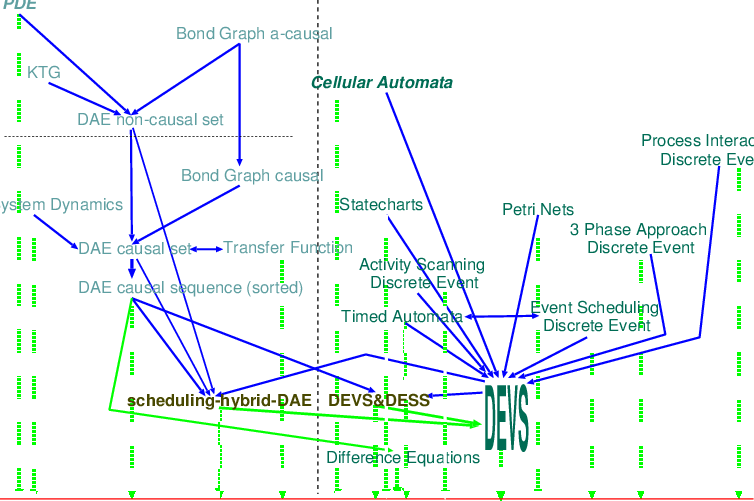
\includegraphics[width=18em]{Formalism-Transformation-Graph-FTG.png}
		\caption{Formalism Transformation Graph (FTG)[1]}
		\label{fig:ftg}
	\end{center}
\end{figure}

Lorum ipsom \ref{fig:ftg}, blah blah.

\FloatBarrier

\subsection{DEVS}


\textit{DEVS is a very powerful super-formalism, but how it's complexity isn't always meaningful when there is a more narrow problem specific formalisum available.}

\textit{DEVS is good, but all of the gory implementation details distracted me from working on what I was actually trying to do, so I designed a layer of abstraction, a problem specific formalism, to make development faster}

\textit{I think that I can probably implement DEVS in terms of my formalism too, should I try/put any time into it?}


\section{My Formalism}

\subsection{Overview}

$I still need a name for this thing, don't I?$

This technique encapsulates the local computation in a territory into a thing called a district. 
A district can represent anything from a house, to a block, to a city or country.
Each district has a way of representing the population of people within it, and any other parameters that change over short spans of time.
Each district also has a way of representing a change in that population. This is something that districts must agree on in order to be connected to one another.
Each district also has it's own computational model for computing the change in that population over time. 
That local computation can use a set of constant parameters to hold information that does not change, stored locally within the district.
Districts also contain the local computation that represents how many people leave the territory over time. This likewise can leverage a set of parameters, this time local to the district and the name of the destination.

It is normal to have many districts in a global model that only vary in the parameters that they store and the connections that they have, though this is not a requirement. The only thing that requires global agreement is the way that districts are identified, and the way that changes in population are represented.

A later development in this project was to add the ability to poke the otherwise constant parameters of a district. This was done to make modelling changes of policy at fixed points in time easier.

\subsection{Formal}

This is the formal description of all of the parts of this formalism that are prescribed. The specifics of all of the listed types are left up to the implementer and modeller other than the fact that the required operations much be well defined over the range of values that come up during simulation.

\begin{verbatim}
<
  ID::TYPE, 
  POP::TYPE, 
  DELTA::TYPE, 
  PARAMS::TYPE, 
  TRAVEL::TYPE, 
  TIME::TYPE,
  
  id::ID, 
  pop::POP, 
  params::PARAMS, 
  travel_rates::MAP<::ID, ::TRAVEL>, 
  
  delta(::PARAMS, ::POP, ::TIME)::DELTA, 
  travel(::TRAVEL, ::POP, ::TIME)::DELTA, 
  add(::POP, ::DELTA)::POP, 
  subtract(::DELTA, ::DELTA)::DELTA
>::DIST

local_advance(dist::DIST, dt::TIME):
| output::MAP<::ID, ::DELTA> = {}
| delta_pop = 
| | dist.delta(dist.params, dist.pop, dt)
| 
| for id, travel in dist.travel_rates:
| | delta_travel = 
| |   dist.travel(travel, dist.pop, dt)
| | 
| | output[id] = delta_travel
| | delta_pop = 
| |   dist.subtract(
| |       delta_pop, 
| |       delta_travel
| |       )
| 
| output[dist.id] = delta_pop
| return output
  
local_apply(
|   dist::DIST, 
|   deltas::SET<::DELTA>
|   ):
| for delta in deltas:
| | dist.pop = 
| |   dist.add(dist.pop, delta)

global_advance(
|   dists::MAP<::ID, ::DIST>, 
|   dt::TIME
|   ):
| messages::MAP<::ID, ::SET<::DELTA>> = {}
| 
| for _, dist in dists:
| | for id, delta in 
| | |   local_advance(dist, dt):
| | | messages[id].add(delta)
| 
| for id, deltas in messages:
| | local_apply(dists[id], deltas)
 
\end{verbatim}

\subsection{PDEVS implementation}

This is the PDEVS implementation that is used in the project so far. It is also prescribed, though again every type within the district that is left to the modeler above is also left to them here.

\begin{verbatim}

Givin some district D, 
the PDEVS atomic model to represent it
is the following

<
  S:{
    id::D.ID,
    pop::D.POP,
    params::D.PARAMS,
    travel_rates::MAP<::D.ID, ::D.TRAVEL>,
    dt::TIME,
    time_till_report::TIME
  },

  X:{
    people_in ::PAIR<::D.ID, ::D.POP>,
    new_params ::PAIR<::D.ID, ::D.PARAMS>,
    new_travel_rate::TUPLE<
        source::D.ID, 
        destination::D.ID, 
        ::D.PARAMS
        >
  },

  Y:{
    report::D.POP,
    people_out::PAIR<::D.ID, ::D.DELTA>
  },

  int:(){
  |   state.time_till_report = state.dt
  },

  ext:(t::TIME, mbs::INPUTS){
  |   state.time_till_report -= t
  |   
  | for src, dest, travel
  | |   in mbs.new_travel_rate:
  | | if state.id == src:
  | | | state.travel_rates[dest] = travel
  |     
  | for id, params in mbs.new_params:
  | | if state.id == id:
  | | | state.params = params
  | 
  | for id, delta in state.people_in:
  | | if state.id = id:
  | | | state.pop = 
  | | |     D.add(state.pop, delta)
  },

  confluent:(t::TIME, mbs::INPUTS){
  | int()
  | ext(0, mbs)
  },
 
  output:(){
  | output = make_output_bags()
  |	
  |	output.report.add(state.pop)
  |	
  | delta = D.delta(
  |     state.params, 
  |     state.pop, 
  |     state.dt
  |     )
  | for dest, travel in state.travel_rates:
  | | tr = D.travel(travel, state.pop, dt)
  | | output.people_out.add(dest, tr)
  | | delta = D.subtract(delta, tr)
  | 
  | output.people_out.add(state.id, delta)
  | 
  | return output
  },

  ta:{
  | return state.time_till_report
  }
>

\end{verbatim}

Each district model \textbf{must} have it's $people\_ou$t connected to it's own $people\_in$. 
For each element in a given district's $travel\_rates$, it \textbf{should} have some model that listens to that element's id connected to that district's $people\_out$. 
There \textbf{should not} be duplicated $id$s, and districts with duplicate $id$s \textbf{must not} be connected.

\section{Results}
\FloatBarrier

\begin{figure}[h!]
	\begin{center}
		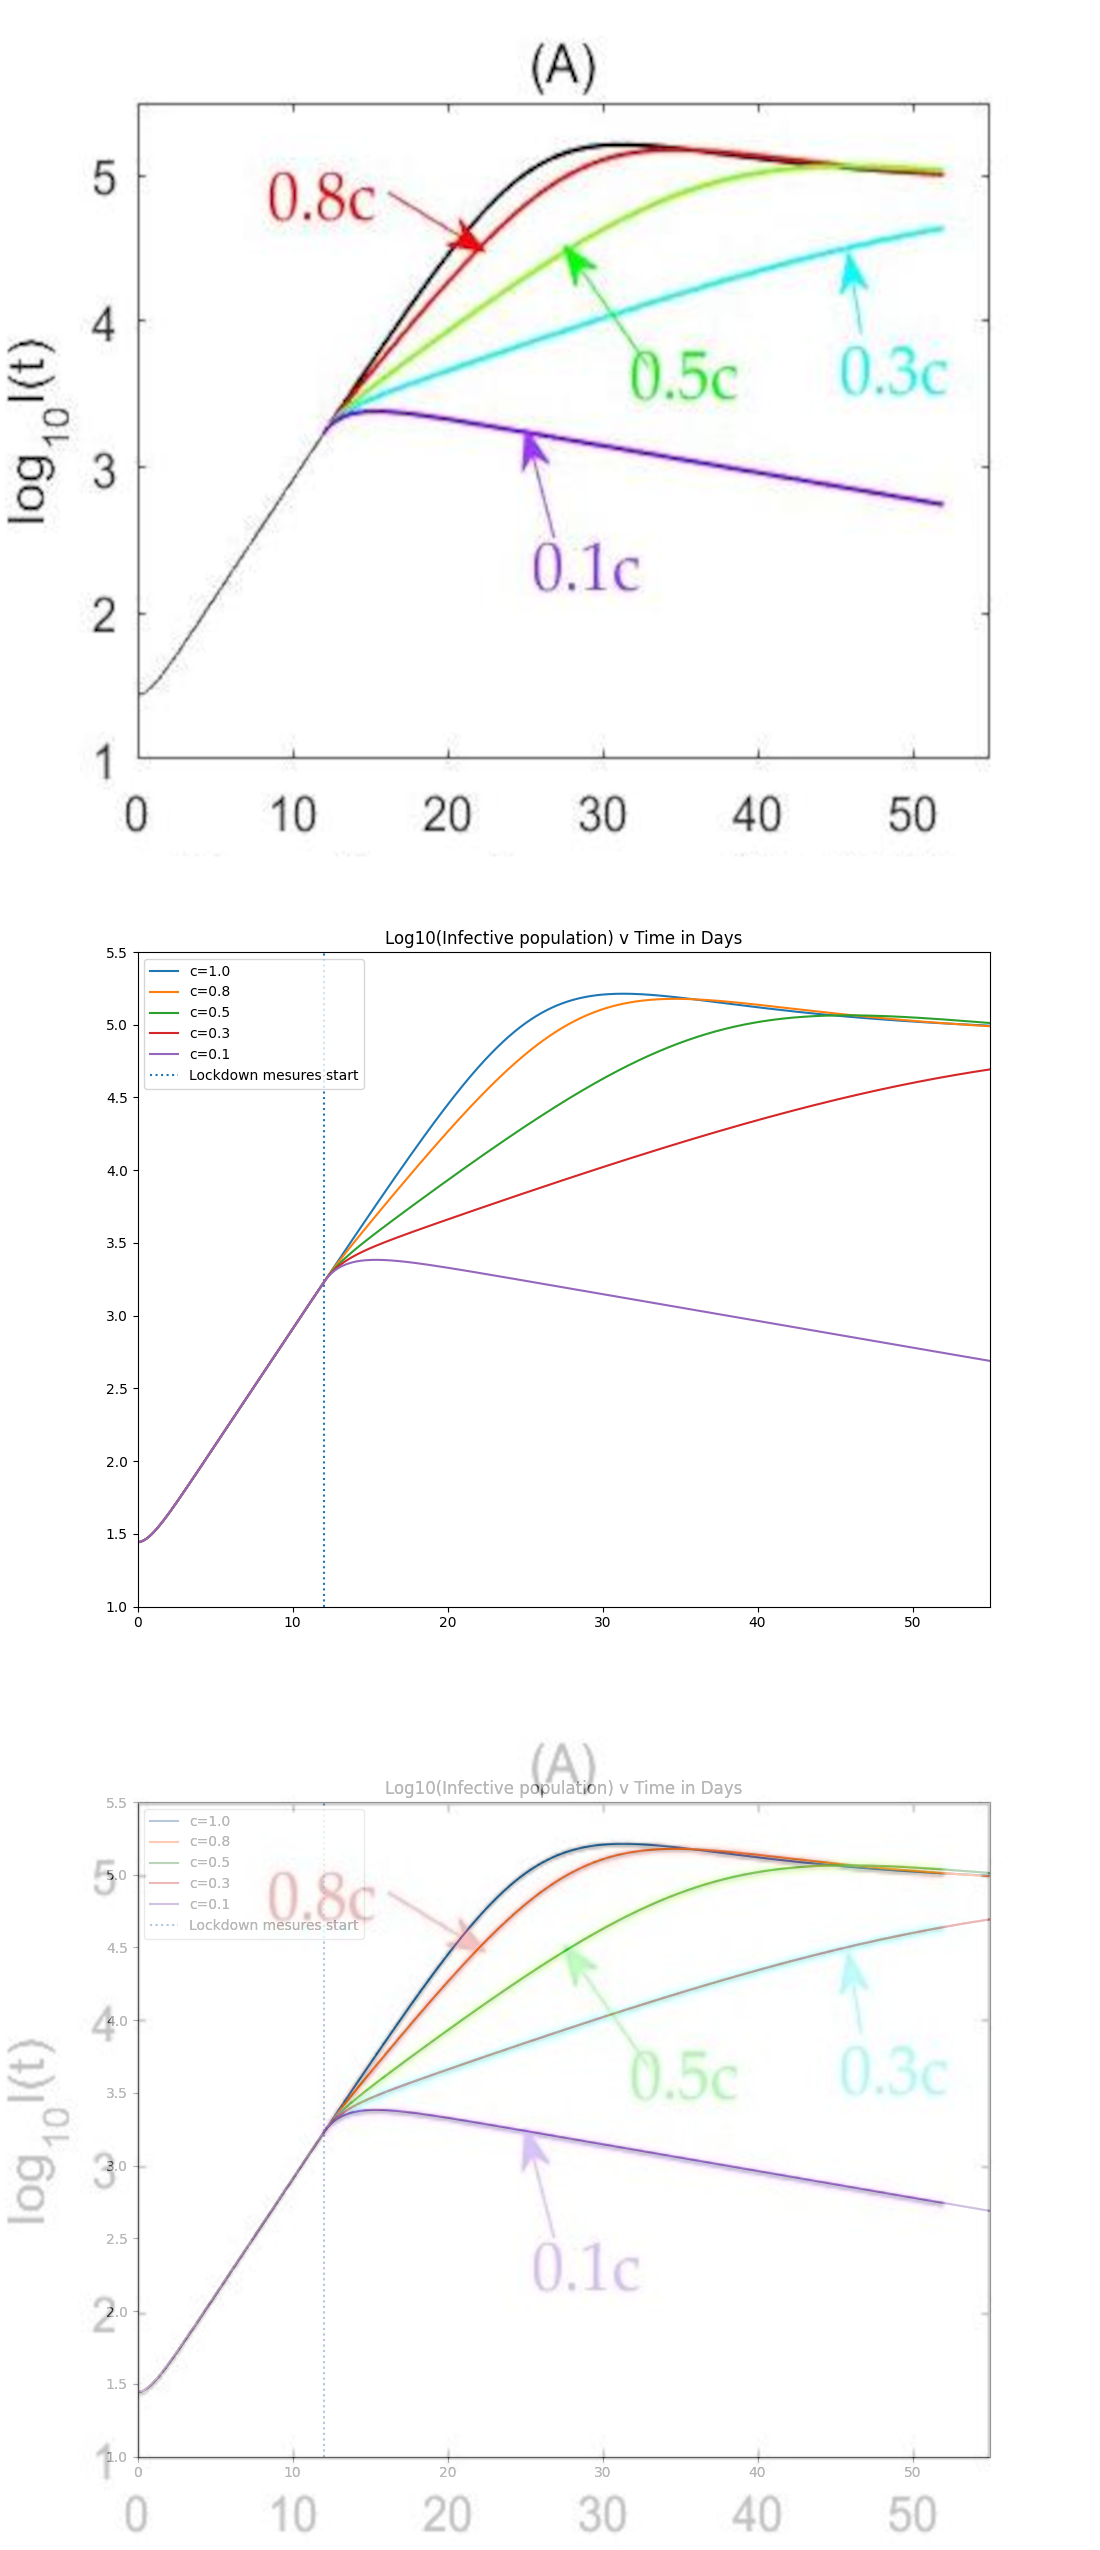
\includegraphics[width=18em]{figure_a_overlay.png}
		\caption{Figure A from original paper[2] (Top), Output from reimplementation (Middle), An overlay to scale of both figures (Bottom)}
		\label{fig:overlay}
	\end{center}
\end{figure}

As we can see in figure \ref{fig:overlay}, blah

\FloatBarrier
\section{Improvements and Future Work}

The current implementation of these tools require that the structure and initial values of the model be hardcoded. This does not represent a fundamental limitation on these techniques, and is an area of future technical development, with the designing of a file format to describe these models and the appropriate parsers and constructors to use this information to lay out a model at run time. 

Another area of development is the formatting of the output. Unlike generalized PDEVS, under the constraints imposed by this formalism, it may be possible to create a generalized and meaningful output parser. The existing $plotter.py$ family of scripts that come bundled with the implementation may be the start of this, or perhaps it will take some other form.

This formalism is compostable, but it is not modular at any scale above a single district. There may be value in also defining a kind of meta district that contains some number of others. It remains to be seen if this will actually be useful at runtime, as opposed to simply flattening the model at construction time, but it should be implemented and tested before it is discarded.

\section{Conclusion}

%This model effectively implements modern ecological connectivity techniques using the Cell-DEVS formalism. This model demonstrates the emergent behaviour present is other sophisticated models, and is relatively simple and straightforward to understand and work with. 

%See \url{https://github.com/xlirate/Cadmin-Cell-DEVS-SAMC} for the code.

\section{Bibliography}

\begin{enumerate}

\item Lara, Juan \& Vangheluwe, Hans. (2002). Computer Aided Multi-paradigm Modelling to Process Petri-Nets and Statecharts. 239-253. 10.1007/3-540-45832-8\_19. \url{http://dx.doi.org/10.1007/3-540-45832-8_19}

\item Tang, B., Wang, X., Li, Q., Bragazzi, N. L., Tang, S., Xiao, Y., \& Wu, J. (2020).
Estimation of the Transmission Risk of the 2019-nCoV and Its Implication for
Public Health Interventions. Journal of clinical medicine, 9(2), 462.
\url{https://doi.org/10.3390/jcm9020462}


%\item Taylor, P. D. et al. 1993. Connectivity is a vital element of landscape
%structure. – Oikos 68: 571–573. \url{
%	https://doi.org/10.2307/3544927 }

%\item Fletcher Jr., R. J. et al. 2011. Social network models predict movement and connectivity in ecological landscapes. – Proc. Natl
%Acad. Sci. USA 108: 19282–19287. \url{https://doi.org/10.1073/pnas.1107549108}
%
%\item Sawyer, S. C. et al. 2011. Placing linkages among fragmented habitats: do least-cost models reflect how animals use landscapes?
%– J. Appl. Ecol. 48: 668–678. \url{https://doi.org/10.1111/j.1365-2664.2011.01970.x}

%\item Beyer, H. L. et al. 2019. Substantial losses in ecoregion intactness highlights urgency of globally coordinated action. – Conservation Letters. 2020; 13:e12692. \url{https://doi.org/10.1111/conl.12692}

%\item Marx, A.J. et al. 2020. samc: an R package for connectivity modeling with spatial absorbing Markov chains. – Ecography, 43: 518-527. \url{https://doi.org/10.1111/ecog.04891}

\end{enumerate}

\end{document}








